\documentclass[12pt,a4paper]{article}
\usepackage{graphicx}
\usepackage{polski}
\usepackage[utf8]{inputenc}
\title{Sprawozdanie z laboratorium PAMSI}
\author{Damian Oleksak}
\date{}
\begin{document}
\maketitle
\newpage

Porównanie czasów pobrania ostatniego elementu z: tablicy asocjacyjnej, tablicy mieszającej i drzewa poszukiwań binarnych.\newline


\includegraphics[scale=0.6]{./asocj}

Wykres 1. Tablica asocjacyjna \newpage


\includegraphics[scale=0.6]{./bst}

Wykres 2. Drzewo poszukiwań binarnych \newpage

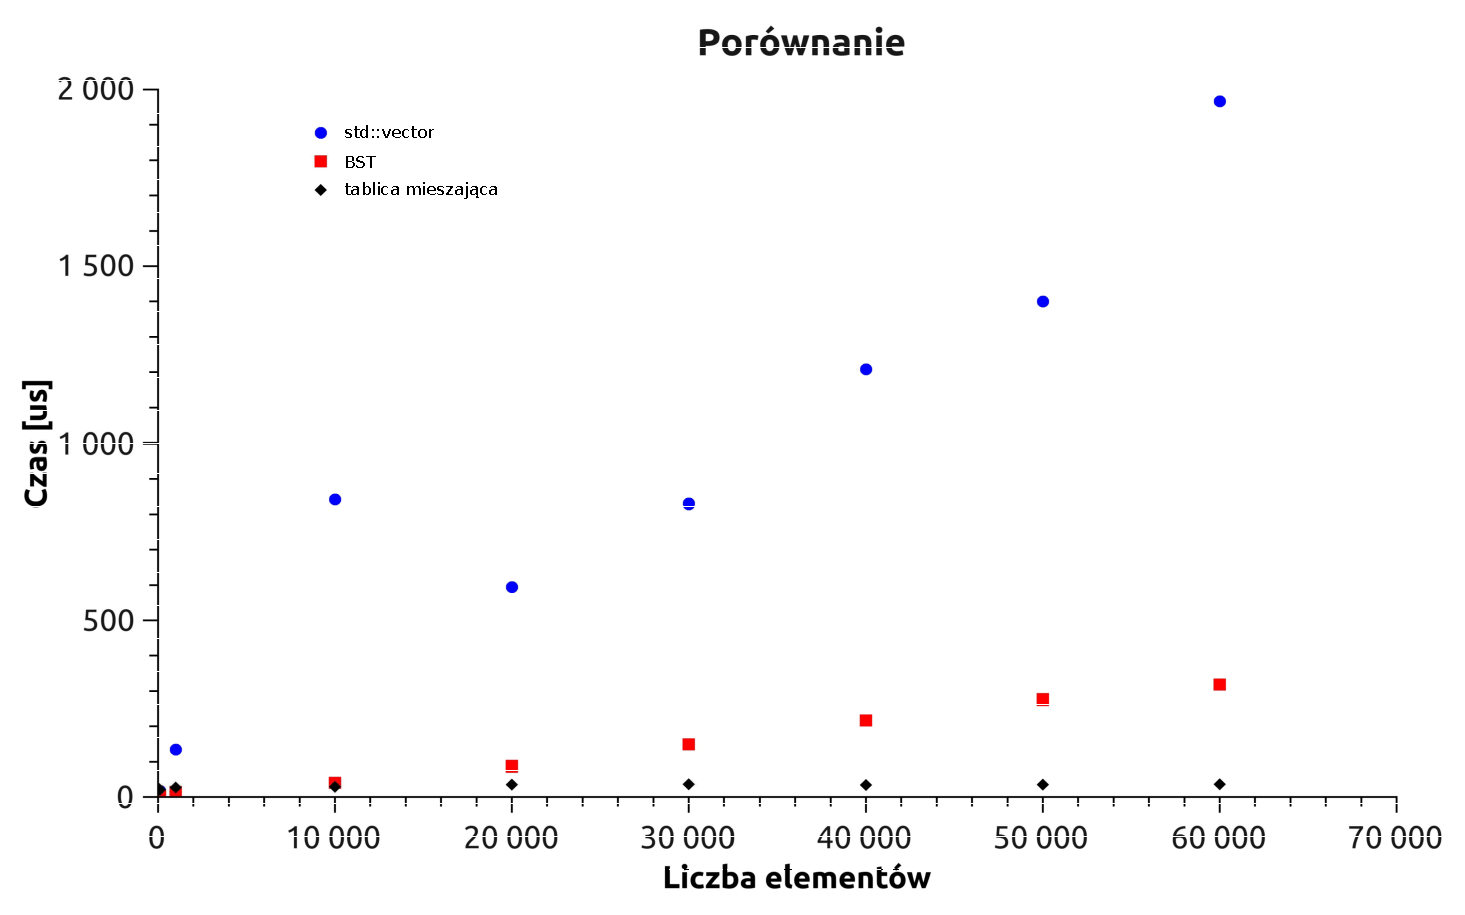
\includegraphics[scale=0.7]{./zb}

Wykres 3. Porównanie \newpage

Wykresy zostały wygenerowane na podstawie pomiarów czasu pobrania ostatniego klucza (o największym numerze indeksu) z n-elementów.    \newline

Sprawozdanie jest jeszcze niekompletne.

\end{document} 
